%============================================================================%
%
%	DOCUMENT DEFINITION
%
%============================================================================%

%we use article class because we want to fully customize the page and don't use a cv template
\documentclass[10pt,A4]{article}	

% Skabelon: https://www.overleaf.com/latex/templates/jan-kusters-left-sidebar-cv/tmmnhrkcmpgv

%----------------------------------------------------------------------------------------
%	ENCODING
%----------------------------------------------------------------------------------------

% we use utf8 since we want to build from any machine
\usepackage[utf8]{inputenc}

%----------------------------------------------------------------------------------------
%	LOGIC
%----------------------------------------------------------------------------------------

% provides \isempty test
\usepackage{xstring, xifthen}

%----------------------------------------------------------------------------------------
%	FONT BASICS
%----------------------------------------------------------------------------------------

% some tex-live fonts - choose your own

%\usepackage[defaultsans]{droidsans}
%\usepackage[default]{comfortaa}
%\usepackage{cmbright}
\usepackage[default]{raleway}
%\usepackage{fetamont}
%\usepackage[default]{gillius}
%\usepackage[light,math]{iwona}
%\usepackage[thin]{roboto} 

% set font default
\renewcommand*\familydefault{\sfdefault} 	
\usepackage[T1]{fontenc}

% more font size definitions
\usepackage{moresize}
% to be able to use ½
\usepackage{textcomp}

%----------------------------------------------------------------------------------------
%	FONT AWESOME ICONS
%---------------------------------------------------------------------------------------- 

% include the fontawesome icon set
\usepackage{fontawesome}

% use to vertically center content
% credits to: http://tex.stackexchange.com/questions/7219/how-to-vertically-center-two-images-next-to-each-other
\newcommand{\vcenteredinclude}[1]{\begingroup
\setbox0=\hbox{\includegraphics{#1}}%
\parbox{\wd0}{\box0}\endgroup}

% use to vertically center content
% credits to: http://tex.stackexchange.com/questions/7219/how-to-vertically-center-two-images-next-to-each-other
\newcommand*{\vcenteredhbox}[1]{\begingroup
\setbox0=\hbox{#1}\parbox{\wd0}{\box0}\endgroup}

% icon shortcut
\newcommand{\icon}[3] { 							
	\makebox(#2, #2){\textcolor{maincol}{\csname fa#1\endcsname}}
}	

% icon with text shortcut
\newcommand{\icontext}[4]{ 						
	\vcenteredhbox{\icon{#1}{#2}{#3}}  \hspace{2pt}  \parbox{0.9\mpwidth}{\textcolor{#4}{#3}}
}

% icon with website url
\newcommand{\iconhref}[5]{ 						
    \vcenteredhbox{\icon{#1}{#2}{#5}}  \hspace{2pt} \href{#4}{\textcolor{#5}{#3}}
}

% icon with email link
\newcommand{\iconemail}[4]{ 						
    \vcenteredhbox{\icon{#1}{#2}{#4}}  \hspace{2pt} \href{mailto:#3}{\textcolor{#4}{#3}}
}

%----------------------------------------------------------------------------------------
%	PAGE LAYOUT  DEFINITIONS
%----------------------------------------------------------------------------------------

% page outer frames (debug-only)
% \usepackage{showframe}		

% we use paracol to display breakable two columns
\usepackage{paracol}

% define page styles using geometry
\usepackage[a4paper]{geometry}

% remove all possible margins
\geometry{top=1cm, bottom=1cm, left=1cm, right=1.5cm}

% fixes a wierd bug where items in itemize environments would break the margin
\usepackage{enumitem}
\setlist{rightmargin=2.5mm}

\usepackage{fancyhdr}
\pagestyle{empty}

% space between header and content
% \setlength{\headheight}{0pt}

% indentation is zero
\setlength{\parindent}{0mm}

% Hyphenation
\hyphenation{en-do-plas-ma-tic}

%----------------------------------------------------------------------------------------
%	TABLE /ARRAY DEFINITIONS
%---------------------------------------------------------------------------------------- 

% extended aligning of tabular cells
\usepackage{array}

% custom column right-align with fixed width
% use like p{size} but via x{size}
\newcolumntype{x}[1]{%
>{\raggedleft\hspace{0pt}}p{#1}}%


%----------------------------------------------------------------------------------------
%	GRAPHICS DEFINITIONS
%---------------------------------------------------------------------------------------- 

%for header image
\usepackage{graphicx}

% use this for floating figures
% \usepackage{wrapfig}
% \usepackage{float}
% \floatstyle{boxed} 
% \restylefloat{figure}

%for drawing graphics		
\usepackage{tikz}				
\usetikzlibrary{shapes, backgrounds,mindmap, trees}

%----------------------------------------------------------------------------------------
%	Color DEFINITIONS
%---------------------------------------------------------------------------------------- 
\usepackage{transparent}
\usepackage{color}

% primary color
\definecolor{maincol}{RGB}{ 50, 100, 250 }

% accent color, secondary
% \definecolor{accentcol}{RGB}{ 250, 150, 10 }

% dark color
\definecolor{darkcol}{RGB}{ 70, 70, 70 }

% light color
\definecolor{lightcol}{RGB}{245,245,245}

% Package for links, must be the last package used
\usepackage[hidelinks]{hyperref}

% returns minipage width minus two times \fboxsep
% to keep padding included in width calculations
% can also be used for other boxes / environments
\newcommand{\mpwidth}{\linewidth-\fboxsep-\fboxsep}
	


%============================================================================%
%
%	CV COMMANDS
%
%============================================================================%

%----------------------------------------------------------------------------------------
%	 CV LIST
%----------------------------------------------------------------------------------------

% renders a standard latex list but abstracts away the environment definition (begin/end)
\newcommand{\cvlist}[1] {
	\begin{itemize}{#1}\end{itemize}
}

%----------------------------------------------------------------------------------------
%	 CV TEXT
%----------------------------------------------------------------------------------------

% base class to wrap any text based stuff here. Renders like a paragraph.
% Allows complex commands to be passed, too.
% param 1: *any
\newcommand{\cvtext}[1] {
	\begin{tabular*}{1\mpwidth}{p{1\mpwidth}}
		\parbox{1\mpwidth}{#1}
	\end{tabular*}
}

%----------------------------------------------------------------------------------------
%	CV SECTION
%----------------------------------------------------------------------------------------

% Renders a a CV section headline with a nice underline in main color.
% param 1: section title
\newcommand{\cvsection}[1] {
	\vspace{14pt}
	\cvtext{
		\textbf{\huge{\textcolor{darkcol}{\uppercase{#1}}}}\\[-4pt]
		\textcolor{maincol}{ \rule{0.1\textwidth}{2pt} } \\
	}
}

%----------------------------------------------------------------------------------------
%	META SKILL
%----------------------------------------------------------------------------------------

% Renders a progress-bar to indicate a certain skill in percent.
% param 1: name of the skill / tech / etc.
% param 2: level (for example in years)
% param 3: percent, values range from 0 to 1
\newcommand{\cvskill}[3] {
	\begin{tabular*}{1\mpwidth}{p{0.72\mpwidth}  r}
 		\textcolor{black}{\textbf{#1}} & \textcolor{maincol}{#2}\\
	\end{tabular*}%
	
	\hspace{4pt}
	\begin{tikzpicture}[scale=1,rounded corners=2pt,very thin]
		\fill [lightcol] (0,0) rectangle (1\mpwidth, 0.15);
		\fill [maincol] (0,0) rectangle (#3\mpwidth, 0.15);
  	\end{tikzpicture}%
}


%----------------------------------------------------------------------------------------
%	 CV EVENT
%----------------------------------------------------------------------------------------

% Renders a table and a paragraph (cvtext) wrapped in a parbox (to ensure minimum content
% is glued together when a pagebreak appears).
% Additional Information can be passed in text or list form (or other environments).
% the work you did
% param 1: time-frame i.e. Sep 14 - Jan 15 etc.
% param 2:	 event name (job position etc.)
% param 3: Customer, Employer, Industry
% param 4: Short description
% param 5: work done (optional)
% param 6: technologies include (optional)
% param 7: achievements (optional)
\newcommand{\cvevent}[7] {
	
	% we wrap this part in a parbox, so title and description are not separated on a pagebreak
	% if you need more control on page breaks, remove the parbox
	\parbox{\mpwidth}{
		\begin{tabular*}{1\mpwidth}{p{0.72\mpwidth}  r}
	 		\textcolor{black}{\Large\textbf{#2}} & \colorbox{maincol}{\makebox[0.25\mpwidth]{\textcolor{white}{#1}}} \\
			\textcolor{maincol}{\textbf{#3}} & \\
		\end{tabular*}\\[8pt]
	
		\ifthenelse{\isempty{#4}}{}{
			\cvtext{#4}
		}
	}

	\ifthenelse{\isempty{#5}}{}{
		\vspace{1pt} %Her stod 9pt før
		{#5}
	}

	\ifthenelse{\isempty{#7}}{}{
		\vspace{1pt} %Her stod 9pt før
		\cvtext{\textbf{Results:}}
		{#7}
	}

	\ifthenelse{\isempty{#6}}{}{
		\vspace{1pt} %Her stod 9pt før
		\cvtext{\textbf{Involved technologies:}}
		{#6}
	}
	\vspace{14pt}
}

%----------------------------------------------------------------------------------------
%	 CV META EVENT
%----------------------------------------------------------------------------------------

% Renders a CV event on the sidebar
% param 1: title
% param 2: subtitle (optional)
% param 3: customer, employer, etc,. (optional)
% param 4: info text (optional)
\newcommand{\cvmetaevent}[4] {
	\textcolor{maincol} {\cvtext{\textbf{\begin{flushleft}#1\end{flushleft}}}}

	\ifthenelse{\isempty{#2}}{}{
	\textcolor{darkcol} {\cvtext{\textbf{#2}} }
	}

	\ifthenelse{\isempty{#3}}{}{
		\cvtext{{ \textcolor{darkcol} {#3} }}\\
	}

	\cvtext{#4}\\[14pt]
}

%---------------------------------------------------------------------------------------
%	QR CODE
%----------------------------------------------------------------------------------------

% Renders a qrcode image (centered, relative to the parentwidth)
% param 1: percent width, from 0 to 1
\newcommand{\cvqrcode}[1] {
	\begin{center}
        \textcolor{maincol}{My LinkedIn}
    \end{center}
	\begin{center}
		
\includegraphics[width={#1}\mpwidth]{qrcode}
	\end{center}
}


%============================================================================%
%
%
%
%	DOCUMENT CONTENT
%
%
%
%============================================================================%
\begin{document}
\columnratio{0.32}
\setlength{\columnsep}{2.2em}
\setlength{\columnseprule}{4pt}
\colseprulecolor{lightcol}
\begin{paracol}{2}
\begin{leftcolumn}
%---------------------------------------------------------------------------------------
%	META IMAGE
%----------------------------------------------------------------------------------------
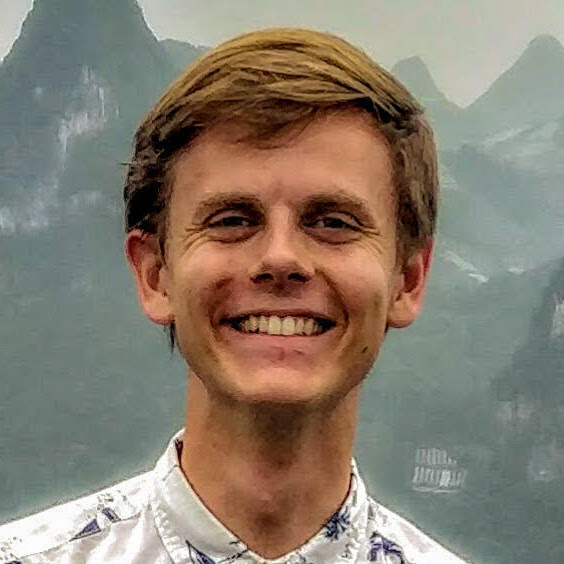
\includegraphics[width=0.94\linewidth]{pb.jpg}	%trimming relative to image size and aligning "FÆRDIGHEDER" with "PROFIL"


%---------------------------------------------------------------------------------------
%	META SKILLS
%----------------------------------------------------------------------------------------
\cvsection{SKILLS}

\cvskill{Teaching}
        {13 yrs} {1} \\[-2pt]

\cvskill{Ski instruction}
        {8 mths} {1} \\[-2pt]

\cvskill{Parkour instruction}
        {5 yrs} {1} \\[-2pt]

\cvskill{Didactics}
        {}{1} \\[-2pt]
        
\cvskill{Communication}
        {} {1} \\[-2pt]

\cvskill{Team work}
        {} {1} \\[-2pt]

% \cvskill{Googling}
%         {20 år} {1} \\[-2pt]

% \cvskill{C\#}
%         {2 år} {0.9} \\[-2pt]
        
% \cvskill{JavaScript}
%         {1 år} {0.9} \\[-2pt]

% \cvskill{TypeScript}
%         {1 år} {0.9} \\[-2pt]
        
% \cvskill{C (ANSI C89)}
%         {1 år} {0.8} \\[-2pt]
        
% \cvskill{Git (CLI)}
%         {2 ½ år} {0.8} \\[-2pt]
        
% \cvskill{Java}
%         {½ år} {0.7} \\[-2pt]
        
% \cvskill{SQL}
%         {2 år} {0.7} \\[-2pt]
        
% \cvskill{Node.js}
%         {1 år} {0.6} \\[-2pt]
        
% \cvskill{Swift}
%         {2 mdr} {0.3} \\[-2pt]

% \cvskill{Software Engineering student}
%         {2 ½ yrs} {0.5} \\[-2pt]
% \newline

% \iconhref{Home}{12}{LasseDS.dk (Portfolio)}{https://lasseds.dk/}{black}\\[6pt]
% \iconhref{Github}{12}{GitHub.com/humleflue}{https://github.com/humleflue}{black}\\[6pt]

\vfill\null
\cvsection{CONTACT ME}\\
\icontext{MapMarker}{12}{Borgmester Jørgensensvej 5\\1st floor, app. 97\\9000 Aalborg, Denmark}{black}\\[6pt]
\iconhref{MobilePhone}{12}{+45 4241 1996}{tel:+4542411996}{black}\\[6pt]
\iconemail{Envelope}{12}{lasse-skaalum@gmail.com}{black}\\[6pt]
\iconhref{Linkedin}{12}{linkedin.com/in/lasse-skaalum}{https://www.linkedin.com/in/lasse-skaalum/}{black}\\[6pt]

% \vfill\null
% \cvqrcode{0.7}

%---------------------------------------------------------------------------------------
%	EDUCATION
%----------------------------------------------------------------------------------------
\newpage
\cvsection{EDUCATION}

\cvmetaevent
{2019 - now}
{B. Sc. Software}
{Aalborg University}
{Studying Software Engineering.}

% \textbf{Course overview (clickable)}
% \setlist{leftmargin=4mm} %reduces the margin for this itemize to make more space
% \cvlist{
%     % 1. semester
%     \item \href
%         {https://moduler.aau.dk/course/2019-2020/DSNDATFB105}
%         {Imperative Programming}
%     \item \href
%         {https://moduler.aau.dk/course/2019-2020/DSNDATFB103}
%         {The Theoretical Foundations of Computer Science (Discrete Mathematics)}
%     % 2. semester
%     \item \href
%         {https://moduler.aau.dk/course/2019-2020/DSNDATFB211}
%         {Algorithms and Data Structures}
%     \item \href
%         {https://moduler.aau.dk/course/2019-2020/DSNDATFB212}
%         {Internetworking and Web-Programming}
%     \item \href
%         {https://moduler.aau.dk/course/2019-2020/DSNDATFB202}
%         {Probability Theory and Linear Algebra}
%     % 3. semester
%     \item \href
%         {https://moduler.aau.dk/course/2019-2020/DSNDATFB311}
%         {Object-Oriented Programming}
%     \item \href
%         {https://moduler.aau.dk/course/2019-2020/DSNDATFB312}
%         {Systems Development (Object-Oriented Analysis & Design)}
%     \item \href
%         {https://moduler.aau.dk/course/2019-2020/DSNDATFB313}
%         {Design and Evaluation of User Interfaces}
%     % 4. semester
%     \item \href
%         {https://moduler.aau.dk/course/2019-2020/DSNDATFB411}
%         {Languages and Compilers}
%     \item \href
%         {https://moduler.aau.dk/course/2019-2020/DSNDATFB412}
%         {Syntax and Semantics}
%     \item \href
%         {https://moduler.aau.dk/course/2019-2020/DSNDATFB413}
%         {Computer Architecture and Operating Systems}
%     % 5. semester
%     \item \href
%         {https://moduler.aau.dk/course/2019-2020/DSNDATFB512}
%         {Agile Software Engineering}
%     \item \href
%         {https://moduler.aau.dk/course/2019-2020/DSNDATFB513}
%         {Machine Intelligence}
%     \item \href
%         {https://moduler.aau.dk/course/2019-2020/DSNDATFB514}
%         {Database Systems}
% }
% \setlist{leftmargin=10mm} % reset the margin of the itemize
% }

% \cvmetaevent
% {2013 - 2016}
% {Studentereksamen (stx)}
% {Silkeborg Gymnasium}
% {Studied in the field of: Biotechnology A, Math A, Physics B.\\
% % Additional topics: Information Technology C
% }

% \cvmetaevent
% {2012 - 2013}
% {Efterskole}
% {Vestbirk Musik- og Sportsefterskole}
% {Student in 10th grade with the majors: Music and vaulting gymnastics.}

\cvmetaevent
{2018}
{Ski Instructor}
{BSI 1}
{Received a week of ski instructor education by \textbf{The Danish Ski School} where I passed all of my exams.\\
\textit{My course certificate is attached.}}

\cvmetaevent
{2015}
{Parkour Instructor}
{DGI's Parkour Instructor Education}
{Received a week of parkour instructor education and passed my exam.}

% \vfill\null
% \cvqrcode{0.7}

%---------------------------------------------------------------------------------------
%	CERTIFICATION
%----------------------------------------------------------------------------------------
\newpage
% \cvsection{COURSES AND CERTIFICATIONS}

% \cvmetaevent
% {2019}
% {Højskoleophold}
% {Forårssemester}
% {Forårssemester på \textbf{Gerlev Idrætshøjskole} med parkour som hovedfag og springgymnastik samt windsurfing som sidefag.}

% \cvmetaevent
% {2016}
% {Master Class Matematik}
% {Master Class Matematik 2016}
% {Deltog i Master Class Matematik 2016, som er et kursus arrangeret af \textbf{Sciencetalenter} for særligt talentfulde elever i 3.g.}

% \vfill\null
% \cvqrcode{0.7}

% \newpage
% \mbox{} % hotfix to place qrcode on the bottom when there are not other elements
% \vfill
% \cvqrcode{0.7}

\newpage
\end{leftcolumn}
\begin{rightcolumn}
%---------------------------------------------------------------------------------------
%	TITLE  HEADER
%----------------------------------------------------------------------------------------
\fcolorbox{white}{darkcol}{\begin{minipage}[c][3.5cm][c]{1\mpwidth}
	\begin {center}
		\HUGE{ \textbf{ \textcolor{white}{ \uppercase{ Lasse D. Skaalum } } } } \\[-24pt]
		\textcolor{white}{ \rule{0.1\textwidth}{1.25pt} } \\[4pt]
		\large{ \textcolor{white} {Software Engineering student with flair for skiing} }
	\end {center}
\end{minipage}} \\[14pt]
\vspace{-12pt}

\textit{Last updated: \today}

%---------------------------------------------------------------------------------------
%	PROFILE
%----------------------------------------------------------------------------------------
\vfill\null
% Make sure no text breaks the margins
\emergencystretch 3em
\cvsection{PROFILE}
\cvtext{I am a thoughtful, energetic and ambitious ski instructor. 
I am a person whom you can always rely on to deliver an extraordinary ski lesson to the clients.\\

I am passionate and dedicated to skiing. 
I have a lot of teaching experience, and despite the fact that most of it has not been ski instruction,
I have developed great didactic and pedagogical skills through these jobs.\\

If you choose to employ me, you will receive a hard-working colleague,
who naturally contributes to the community. You can expect a resource,
who always does his best to give the clients the best skiing experience,
who always is fit to work in the mornings,
and who is always open to constructive feedback.\\

\textit{I have more teaching experience than what I have put in the "WORK EXPERIENCE" section, which I have omitted in an attempt not to bloat the CV more than necessary.\\
The rest of my work experience can be found on my \href{https://www.linkedin.com/in/lasse-skaalum/}{LinkedIn}, but in short it includes teaching in primary school, home work helper, parkour instructor and drum teacher.}
}

%----------------------------------------------------------------------------------------
%	WORK EXPERIENCE
%----------------------------------------------------------------------------------------
\vfill\null
\cvsection{WORK EXPERIENCE}

% \cvevent
% 	{June 21 - now}
% 	{Student Programmer}
% 	{Trifork}
% 	{Student Programmer at the software innovation company Trifork, where I help the consultants solve various tasks related to programming.}
% 	{
%         % \cvlist{
% 	    % \item Modelling of a HR-related domain both on database and backend level.
% 	    % \item API design and implementation.
% 	    % }
%     }%Arbejdsopgaver
% 	{
%         % \cvlist{
% 	    % \item C\#
% 	    % \item ASP.NET Core
% 	    % \item ASP.NET Web API
% 	    % \item OpenAPI (Swagger)
% 	    % \item Entity Framework Core
% 	    % \item Microsoft SQL Server
% 	    % \item Azure Cosmos DB
% 	    % \item TypeScript
% 	    % \item Azure DevOps
% 	    % \item Swift
% 	    % \item Kotlin
% 	% }
%     }%Involverede teknologier
% 	{
%         % \cvlist{
% 	    % \item Reddede en stor demo for en af Danmarks største virksomheder fra at gå i vasken på morgenen, hvor demoen skulle finde sted, ved at lave et hotfix. Et af dependenciesne var uheldigvis tagget med \texttt{:latest}, hvilket havde fået hele systemet til at bryde sammen efter en softwareopdatering aftenen forinden.
% 	    % }
%     }%Resultater

\cvevent
	{May 21 - now}
	{Mentor}
	{Aalborg Universitet}
	{Mentoring a software engineering student. I am helping the student both with academic stuff as well as social stuff.\\
    }
	{}%Arbejdsopgaver
	{}%Involverede teknologier
	{\cvlist{
	    \item My mentee has ambitions to become the best in our field, so I have of course done my very best to make him succeed in this regard. This has resulted in multiple top marks, which he has been very proud of.
	    \item My mentee has given me a Christmas present on his own initiative.
	}}%Resultater

\cvevent
	{Sep 20 - June 21}
	{Teaching Assistant}
	{Aalborg University}
	{Teaching Assistant in "Imperative Programming" and "Algorithms and Data Structures".}
	{\cvlist{
	    \item Helped the university students with their assignments after the lectures.
	    \item Corrected the student's assignments and gave them constructive feedback.
	    \\\\\textit{A recommendation from the lecturer can be sent on request (in Danish).}
	}}%Arbejdsopgaver
	{
        % \cvlist{
	    % \item C (Programming Language)
	    % }
    }%Involverede teknologier
	{\cvlist{
	    \item One of the students contacted me privately and expressed his satisfaction with my help in the course. In continuation hereof, he asked me if I wanted to become his mentor. I thought it sounded exciting, and therefore I said yes to the opportunity.
	}}%Resultater

\cvevent
	{July 20 - Nov 20}
	{Rus Instructor}
	{Aalborg Universitet}
	{Was in charge of planning and carrying out social activities during the commencement of the new software engineering students.}
	{
        % \cvlist {
	    % \item Was the driving force behind streaming our LAN-event, which involved planning the event, setting up the streaming software and finally streaming messages and game play during the weekend of the event.
	    % \item Had six of my fellow students help me during the weekend of the event, whom I collaborated with, to make the event a success.
	    % }
    }%Arbejdsopgaver
	{}%Involverede teknologier
	{
        % \cvlist{
	    % \item Prior to the event I managed to gather sponsorships each valuing up to 10.000 DKK. The sponsors included companies like CEGO, Red Bull, BankData and PROSA. The money was spent on making the event extra special with goodie bags for all participants and prices for the tournament winners.
	    % }
    }%Resultater

\cvevent
	{Maj 20 - Jun 20}
	{Programming Teacher}
	{Silkeborg Ungdomsskole}
	{Introduced a group of young students to basic web programming}
	{\cvlist {
	    \item Planned and carried out the course all by myself.
	}}%Arbejdsopgaver
	{
        % \cvlist {
	    % \item HTML, CSS og JavaScript.
	    % \item Discord (Undervisningen foregik virtuelt pga. coronaepedimien).
	    % }
    }%Involverede teknologier
	{}%Resultater

\cvevent
	{Nov 18 - Feb 19}
	{Ski Instructor}
	{Niseko Village Snow School}
	{Taught skiing to people of all ages and levels.}
	{\cvlist {
	    \item Instruction of all ages and skill levels.
	    \item Snow clearing in the mornings.
	    \item Setup of the kids area.
	    \\\\\textit{The ski school's end of season review is attached.}
	}}%Arbejdsopgaver
	{}%Involverede teknologier
	{}%Resultater

% \cvevent
% 	{Jan 17 - Nov 18}
% 	{Lærervikar}
% 	{Dybkærskolen}
% 	{Underviste børn og unge på folkeskoleniveau. Blev gradvist kaldt ind oftere og endte med at blive kaldt ind hver dag det sidste år af min ansættelse.}
% 	{\cvlist {
% 	    \item Underviste i alle fag på alle klassetrin.
% 	    \item Faste lektioner i en periode på et halvt år i en modtagerklasse, hvor jeg udarbejdede mit eget. undervisningsmateriale\\\textbf{Fag:} Kulturfag.
% 	    \item Faste lektioner i en periode på et halvt år i en 3. klasse.\\\textbf{Fag:} Musik, bibliotek og lektielæsning.
% 	    \item Påtog mig det fulde ansvar og sikrede dermed en god kvalitet af undervisningen på trods af lærerens fravær.
% 	    \\\\\textit{Udtalelse fra skolen kan tilsendes, hvis det ønskes.}
% 	}}%Arbejdsopgaver
% 	{}%Involverede teknologier
% 	{}%Resultater
	
% \cvevent
% 	{Aug 17 - Nov 18}
% 	{Pædagogmedhjælper}
% 	{Dybkærklubben}
% 	{Arbejdede både i klubbens fritidsafdeling og ungdomsafdeling. Havde fleksible arbejdstider, men arbejdede gennemsnitligt 18 timer ugentligt.}
% 	{\cvlist {
% 	    \item Ansvarlig for al IT i klubben (Playstation, PCer, Wii mv.).
% 	    \item Ansvarlig for gymnastiksalen.
% 	    \\\\\textit{Reference fra klubben kan tilsendes, hvis det ønskes.}
% 	}}%Arbejdsopgaver
% 	{}%Involverede teknologier
% 	{}%Resultater

% \cvevent
% 	{Sep 17 - Sep 18}
% 	{Pædagogmedhjælper}
% 	{Myretuen SFO}
% 	{Vikarierede i tilfælde af pædagogernes fravær, samt hvis klubben manglede mandskab til udflugter.}
% 	{}%Arbejdsopgaver
% 	{}%Involverede teknologier
% 	{}%Resultater
	
% \cvevent
% 	{Aug 17 - Aug 18}
% 	{Lektiehjælper}
% 	{Privat}
% 	{Hjalp tre børn/unge, som aldersmæssigt spændte fra 4. klasse til 1.g, med deres lektier.}
% 	{}%Arbejdsopgaver
% 	{}%Involverede teknologier
% 	{}%Resultater
	
% \cvevent
% 	{Aug 14 - Jun 18}
% 	{Parkourtræner}
% 	{Silkeborg Ungdomsskole}
% 	{Trænede op til fire hold om ugen 2 timer pr. hold.}
% 	{\cvlist {
% 	    \item Planlagde og udførte undervisning på ugentlig basis.
% 	    \item Planlagde og udførte parkourture til flere destinationer i Danmark.
% 	}}%Arbejdsopgaver
% 	{}%Involverede teknologier
% 	{\cvlist {
% 	    \item Boostede parkourmiljøet i Silkeborg. I min tid som instruktør gik vi fra et ugentligt hold i Silkeborg Kommune til fire.
% 	}}%Resultater
	
% \cvevent
% 	{Somrene 15 \& 17}
% 	{Delikatesseassistent (15)\hfill \break Salgsassistent (17)}
% 	{Føtex Ebeltoft}
% 	{Sommerferiejob i Føtex Ebeltoft, hvor jeg hjalp butikken pga. det ekstra pres i sommerferien.}
% 	{}%Arbejdsopgaver
% 	{}%Involverede teknologier
% 	{}%Resultater
	
% \cvevent
% 	{Sep 14 - Maj 15}
% 	{Parkourtræner}
% 	{Ungdomsskolen Favrskov}
% 	{Trænede et hold i Hinnerup en gang om ugen i 2 timer.}
% 	{\cvlist {
% 	    \item Planlagde og udførte undervisning på ugentlig basis.
% 	    \item Samlede en del af holdet op i Hammel og kørte dem i minibus til Hinnerup, så de også kunne deltage i træningen.
% 	}}%Arbejdsopgaver
% 	{}%Involverede teknologier
% 	{}%Resultater
	
% \cvevent
% 	{Sep 11 - Sep 14}
% 	{Servicemedarbejder}
% 	{Føtex Nørrevænget}
% 	{Servicemedarbejder i kolonialafdelingen.}
% 	{}%Arbejdsopgaver
% 	{}%Involverede teknologier
% 	{}%Resultater

% \cvevent
% 	{Sep 08 - Jun 12}
% 	{Trommelærer}
% 	{Privat}
% 	{Trommelærer for fire børn på ca. 9 år.}
% 	{\cvlist {
% 	    \item Planlagde og udførte undervisning på ugentlig basis.
% 	    \item Udarbejdede mit eget undervisningsmateriale.
% 	}}%Arbejdsopgaver
% 	{}%Involverede teknologier
% 	{}%Resultater
	
%----------------------------------------------------------------------------------------
%	FRIVILLIGE GØREMÅL
%----------------------------------------------------------------------------------------
% \vfill\null
\cvsection{VOLUNTEERING}

% \cvevent
% 	{Dec 20 - nu}
% 	{Formand}
% 	{ABK-Net}
% 	{Formand for netforeningen på Arbejderbevægelsens Kollegium, hvor jeg bor.\\
% 	Vi har ansvaret for alle 198 lejligheders internet, kollegiets hjemmeside samt kollegiets mailservice. Dette indebærer håndtering af sikkerhed samt vedligeholdelse af systemerne.\\
% 	Læs mere her: \url{https://abk-aalborg.dk/page/board/abk-net/}\\
% 	GitLab: \url{https://gitlab.com/abk-aalborg}
% 	}
% 	{}%Arbejdsopgaver
% 	{\cvlist{
% 	    \item NixOS
% 	    \item Grafana
% 	}}%Involverede teknologier
% 	{\cvlist{
% 	    \item Kollegiets hjemmeside: \url{https://abk-aalborg.dk/}
% 	    \item Under mit formandsskab formåede vi at opsætte netværket på ny helt fra bunden af. Det involverede køb samt opsætning af udstyret. Det resulterede i en opgradering af hver kollegianers internetforbindelse fra 100 Mbit til 1 Gbit. Derudover sørgerede vi for at dokumentere det hele grundigt, så fremtidige netforeningsmedlemmer har en chance for at vedligeholde systemet.
% 	}}%Resultater

\cvevent
	{Feb 18 - now}
	{Ski Instructor}
	{Silkeborg Ski Club}
	{Instructing on my home town's skiing club's ski trips.}
	{}%Arbejdsopgaver
	{}%Involverede teknologier
	{}%Resultater
	
\cvevent
	{Jan 20 - now}
	{Ski Instructor}
	{Harreskov Ski Club}
	{Instructing on the club's ski trips.}
	{}%Arbejdsopgaver
	{}%Involverede teknologier
	{}%Resultater

\cvevent
	{Sep 20 - now}
	{Tutor}
	{Aalborg Universitet}
	{Making sure that new software students have a great start at the university.}
	{}%Arbejdsopgaver
	{}%Involverede teknologier
	{}%Resultater

% \cvevent
% 	{Oct 20 - nu}
% 	{Bestyrelsesmedlem}
% 	{ABK-Beboerråd}
%     {Aktivt medlem af beboerrådet på Arbejdserbevægelsens Kollegium, hvor jeg bor.\\
% 	Læs mere her: \url{https://abk-aalborg.dk/page/board/council/}}
% 	{}%Arbejdsopgaver
% 	{}%Involverede teknologier
% 	{}%Resultater

% \cvevent
% 	{Aug 20 - Dec 20}
% 	{Bestyrelsesmedlem}
% 	{ABK-Net}
% 	{}
% 	{}%Arbejdsopgaver
% 	{}%Involverede teknologier
% 	{}%Resultater

% \cvevent
% 	{Aug 16 - Sep 16}
% 	{Engelsklærer}
% 	{Love Volunteers}
% 	{Arbejdede i en kinesisk børnehave i 6 uger.
% 	\\\\\textit{Min koordinators vurdering af min indsats kan tilsendes, hvis det ønskes.}}
% 	{}%Arbejdsopgaver
% 	{}%Involverede teknologier
% 	{}%Resultater
	
% \cvevent
% 	{Dec 13 - Dec 15}
% 	{Formand}
% 	{Silkeborg Gymnasiums IKT-udvalg}
% 	{Formand for Silkeborg Gymnasium Elevråds Informations- og Kommunikationsteknologiske udvalg.}
% 	{}%Arbejdsopgaver
% 	{}%Involverede teknologier
% 	{}%Resultater

% \cvevent
% 	{Okt 13 - Jun 16}
% 	{Elevrådsrepræsentant}
% 	{Silkeborg Gymnasiums elevråd}
% 	{Deltog aktivt som elevrådsrepræsentant i Silkeborg Gymnasiums elevråd.}
% 	{}%Arbejdsopgaver
% 	{}%Involverede teknologier
% 	{}%Resultater
	
\cvevent
	{Sep 13 - Maj 14}
	{Parkour Instructor}
	{Silkeborg Ungdomsskole}
	{Instructed a parkour team once a week for 2 hours.
	\\\\\textit{My boss' assessment of my work can be sent on request (in Danish).}}
	{}%Arbejdsopgaver
	{}%Involverede teknologier
	{}%Resultater

% hotfixes to create fake-space to ensure the whole height is used
% \mbox{}
% \vfill
% \mbox{}
% \vfill
% \mbox{}
% \vfill
% \mbox{}
\end{rightcolumn}
\end{paracol}
\end{document}

